
%This chapter is for providing the context to your panelist/reader.  It is actually an expanded form of the Background of the Study that you have put in Chapter~\ref{ch:intro}.

To start, computer vision plays an important and pivotal role in machine learning as it equips machines and other systems with the ability to perceive, interpret and understand visual information from our physical environment. Equipping computer systems with this human-like vision capability can be very helpful in many applications such as autonomous driving, advanced medical image analysis and many more. One of the most basic yet very critical functions of computer vision is to process and analyze images to detect and classify objects. This is one of the most important attributes of vision as it can be very useful once computers can correctly recognize and identify different objects. This is where machine learning algorithms further improve its significance. As these computer vision models are exposed to more visual data and information, it can improve in terms of its accuracy and correctness when it comes to identifications and even predictions. This adaptability can be very critical on the performance of these machine vision models in different settings with different lighting conditions which can effectively alter image quality.  

\begin{figure}[!htbp]
	\centering
		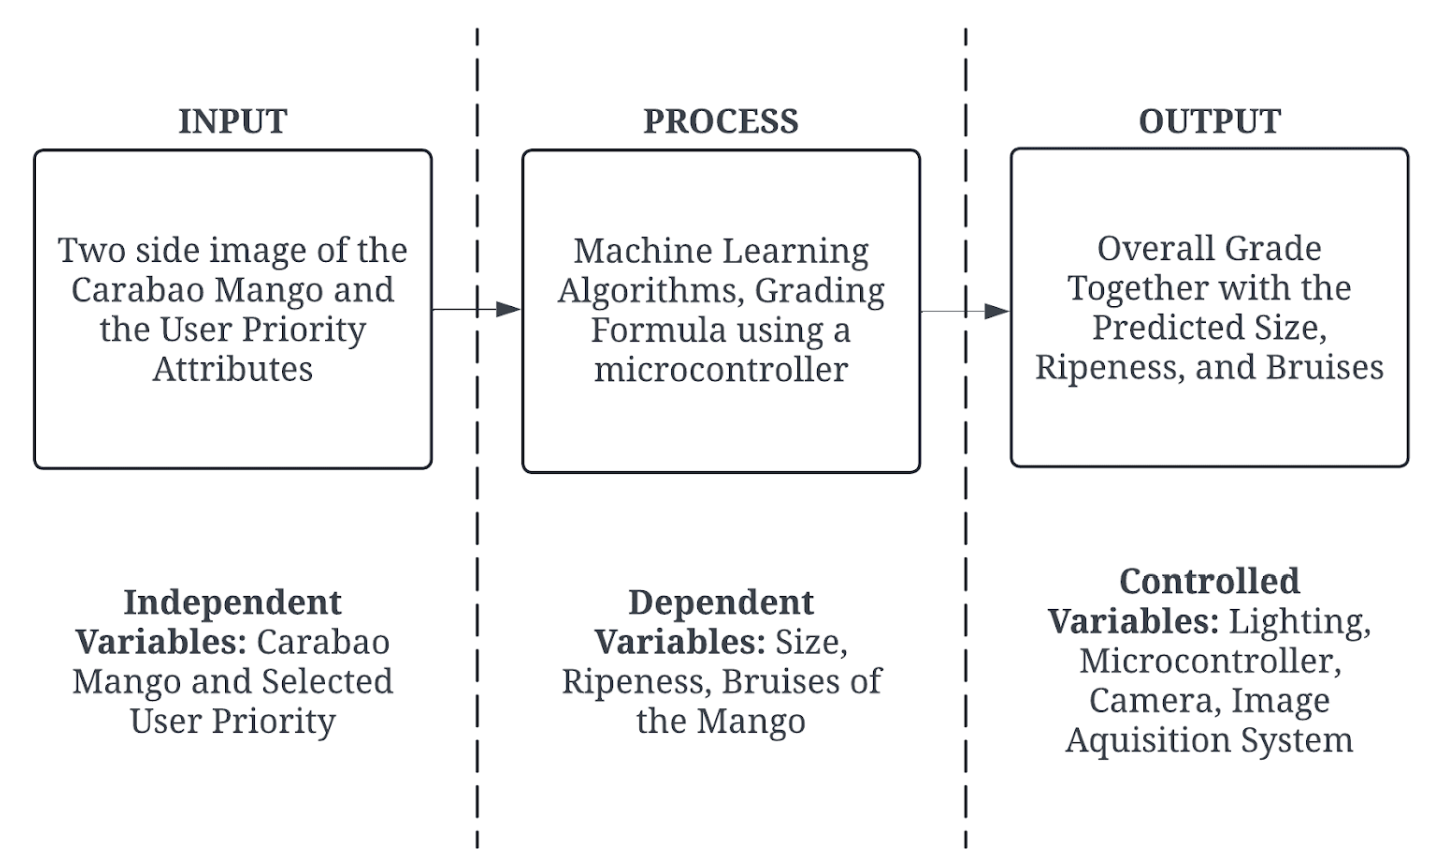
\includegraphics[width=0.9\textwidth]{conceptdiagram}
	\caption{Conceptual Framework }
	\label{fig:conceptdiagram}
\end{figure}

\section{Summary}

Provide the gist of this chapter such that it reflects the contents and the message.